% xelatex %
%
\documentclass[10pt, a4paper ]{article}

\PassOptionsToPackage{usenames, dvipsnames, xetex}{xcolor}

\usepackage[frenchb]{babel}
\usepackage{fontspec}
% \pagestyle{empty}
\usepackage{marvosym}
\usepackage{dice}

% DOCUMENT LAYOUT
\usepackage{geometry}
\geometry{a4paper, textwidth=5.5in, textheight=8.5in, marginparsep=7pt,
marginparwidth=.6in}

\setlength\parindent{3mm}
\setlength\parskip{3mm}

% \definecolor{MidnightBlue}{rgb}{0.15,0.30,0.55}
% \definecolor{BrickRed}{rgb}{0.55,0.15,0.30}
% \usepackage[usenames,xetex]{color}

% FONTS
\usepackage{xunicode}
\usepackage{xltxtra}
\usepackage{amsmath}

% converts LaTeX specials (``quotes'' --- dashes etc.) to unicode
\defaultfontfeatures{Mapping=tex-text}

\setromanfont [Ligatures={Common}%, Numbers={OldStyle}
]{Gentium Basic}
\setsansfont [Ligatures={Common}, BoldFont={Fontin Sans Bold},
ItalicFont={Fontin Sans Italic}]{Fontin Sans}
\setmonofont[Scale=0.8]{Monaco}

% PDF SETUP
\usepackage[xetex, bookmarks, colorlinks, breaklinks, pdftitle={Rendu d'images
3D par lancer de rayons}, pdfauthor={Xavier Olive}]{hyperref}
\hypersetup{linkcolor=MidnightBlue,citecolor=BrickRed,
filecolor=black,urlcolor=MidnightBlue}

\title{Rendu d'images 3D par lancer de rayons}
\begin{document}

\noindent
\textbf{\textsf{\large IN 104 -- Rendu d'images 3D par lancer de rayons }}
\vskip1mm\hrule%\url{www.xoolive.org}

% \maketitle

\begin{minipage}{.9\textwidth} \sf L'objectif de ce projet est de concevoir et
    développer un projet logiciel complet capable de synthétiser des images par
    lancer de rayons. L'accent sera mis sur la découverte de méthodes de travail
    couramment utilisées dans le monde industriel.  \end{minipage}

% \tableofcontents

\section{Principe général}

Le logiciel à écrire est un logiciel de synthèse d'images. Il s'agit
de produire l'image que pourrait voir un observateur placé à un certain
point et qui regarderait une scène modélisée dans son champ de vision avec un
éclairage particulier.

Le lancer de rayons est la manière historique de produire des images 3D. C'est
un excellent moyen de rendre compte des caractéristiques géométriques de la
lumière. (réflexion, réfraction, transparence) Aujourd'hui, d'autres méthodes
existent pour gérer la 3D (OpenGL, CG), mais le lancer de rayons reste néanmoins
un sujet d'actualité.

Le logiciel demandé ici ne traitera que d'un cas simplifié avec une seule source
de lumière. Seuls les couleurs propres des objets et le phénomène de réflexion
seront pris en compte.

\begin{figure}[h]
    \centering
    \hfill
    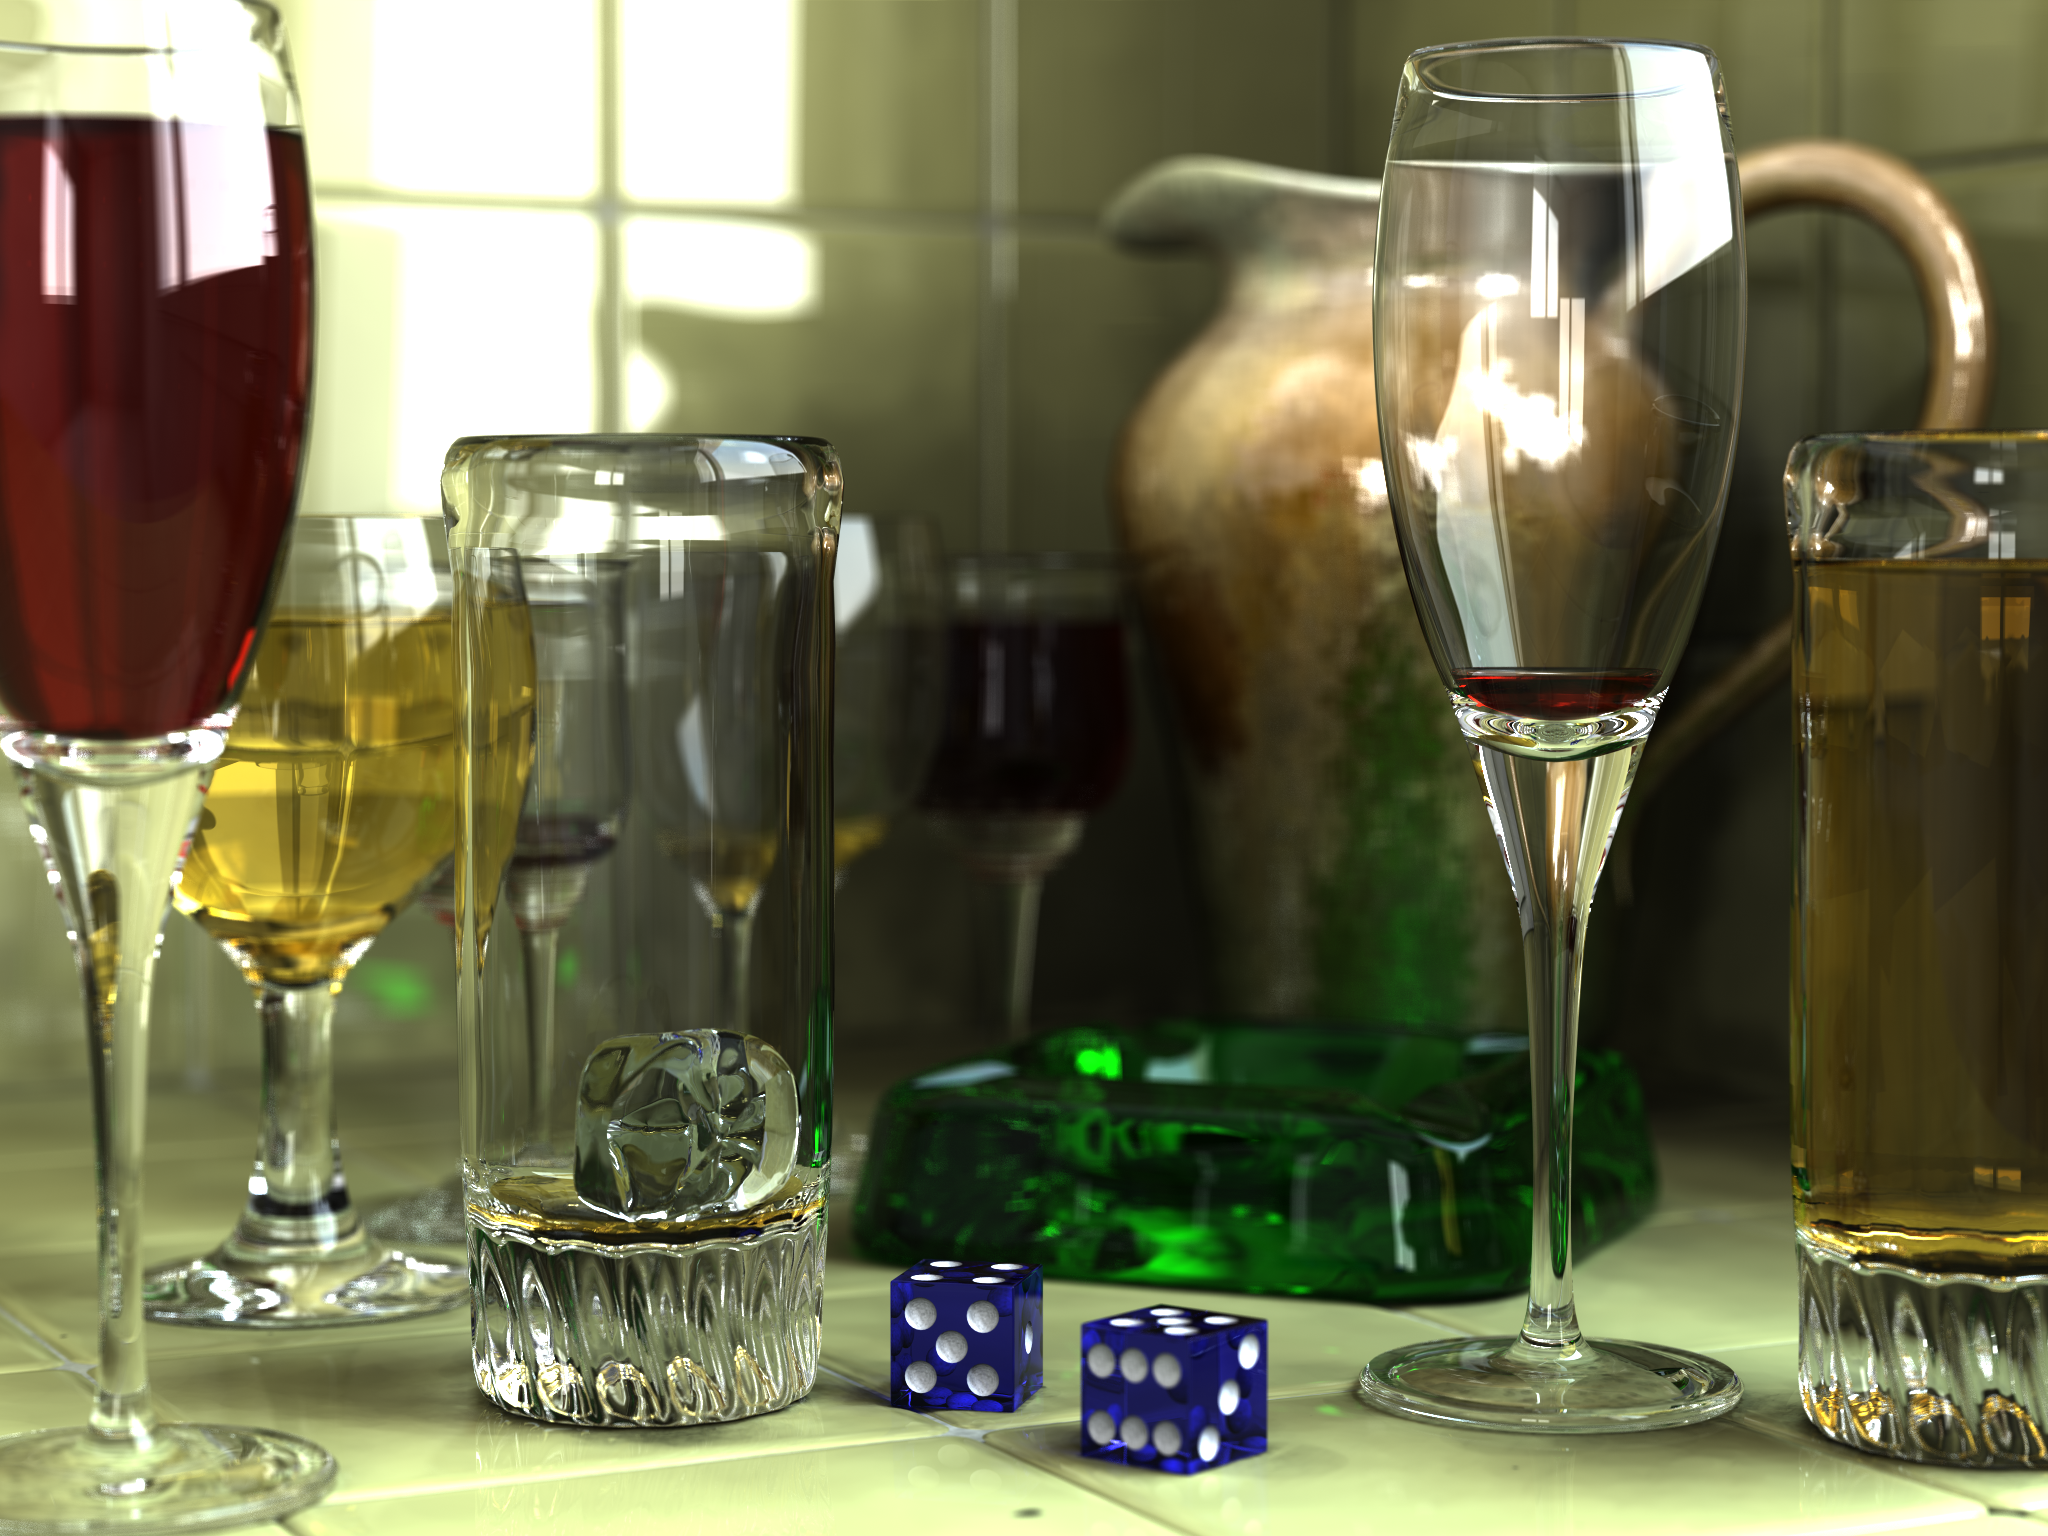
\includegraphics[width=.40\textwidth] {../../img/glass_dice.png}
    \hfill
    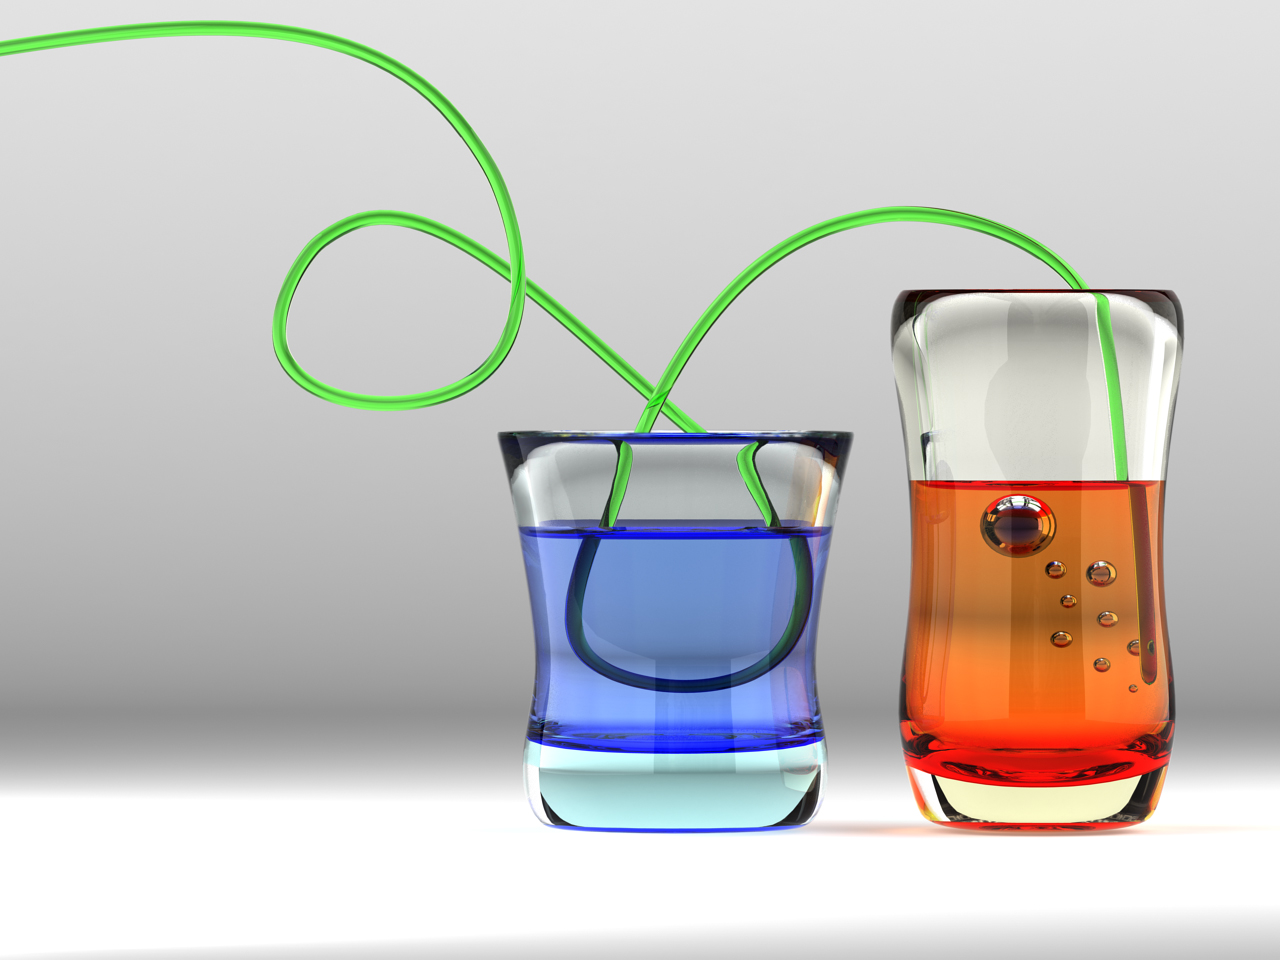
\includegraphics[width=.40\textwidth] {../../img/glass_straw.png}
    \hfill\mbox{}
    \caption{Exemples d'images rendues par un lancer de rayon}
    \label{fig:sample}
\end{figure}


\section{Méthode de travail}

Le logiciel devra répondre à des exigences de qualité décrites pendant les
séances. Les étudiants seront notamment encouragés à suivre un processus de
développement itératif, à produire et valider des tests unitaires, à écrire une
documentation et à fournir un code source autosuffisant pour la compilation et
l'exécution (Makefile).

Dans un second temps, vous serez encouragés à explorer une piste d'étude de
votre choix autour de la version basique développée. L'étude sera
essentiellement théorique (rapport écrit) mais pourra aussi être accompagnée de
code dans le but d'illustrer votre propos. Les pistes d'exploration seront
libres mais pourront aussi être choisies parmi une liste fournie.

Les études pourront concerner la prise en compte de sources de lumière
multiples, de la transparence, de la réfraction, ou de la profondeur de champ.
Elles pourront également concerner la complexité algorithmique ou des
traitements à la limite du champ d'application du lancer de rayon
(anti-crénelage, application de textures, \ldots)

\section{Notation}

En plus de la livraison d'un exécutable (sous la forme répertoire source et
fichier Makefile), les étudiants devront rendre un rapport qui analyse leur
expérience du projet. Celui-ci sera complété par un descriptif de la
méthodologie choisie et des difficultés rencontrées pour le développement. Il
contiendra également les résultats de l'étude.

Le barème d'évaluation est décrit ci-dessus.

\begin{table}
    \centering
    \begin{tabular}[hb]{|lcl|}
        \hline
        \textbf{Règles et bonnes pratiques} && 2 points\\\hline
        Code indenté, commenté; bonnes pratiques && 1 point\\
        Respect d'un développement itératif &$\star$& 1 point \\\hline\hline
        \textbf{Tests unitaires} && 3 points\\\hline
        Note rendue par le programme de test fourni && 2 points\\
        Écriture de ses propres tests & $\star$  & 1 point\\\hline\hline
        \textbf{Livraison de la fourniture} && 4 points\\\hline
        Code qui ne compile pas (tests ou exécutable) && {\color{red} -2 points}\\
        Lancer de rayon fonctionnel & $\star$ & 2 points\\
        Lecture de fichier d'entrée && 1 point\\
        Production de fichier de sortie && 1 point\\\hline\hline
        \textbf{Étude d'une problématique choisie} & $\star$ & 4 points\\\hline
        Définition du problème étudié & $\star$ & 1 point \\
        Analyse du problème & $\star$ & 3 points \\
        Bonus difficulté & $\star$ & +1 point \\\hline\hline
        \textbf{Analyse de la pratique} & $\star$ & 4 points\\\hline\hline
        \textbf{Soutenance} & & 4 points\\\hline
        Fond et forme seront notés à pondération égale &&\\\hline\hline
        \textbf{Pénalité de retard} & & 10\,\%\\\hline

    \end{tabular}

    \caption{Barème de notation. Les items marqués du symbole $\star$ doivent
    faire l'objet d'une analyse dans le rapport. Ils seront évalués au moins
partiellement, sinon entièrement,  au regard de celui-ci.}

    \label{tab:bareme}
\end{table}



\end{document}
